\documentclass[11pt]{article}
\usepackage[margin=1in, top=1in]{geometry}
\usepackage[all]{nowidow}
\usepackage[hyperfigures=true, hidelinks, pdfhighlight=/N]{hyperref}
\usepackage[separate-uncertainty=true, group-digits=false]{siunitx}
\usepackage{graphicx,amsmath,physics,tabto,float,amssymb,pgfplots,verbatim,tcolorbox}
\usepackage{listings,xcolor,subfig,caption,import,wrapfig,biblatex}
\usepackage[version=4]{mhchem}
\usepackage[noabbrev]{cleveref}
\newcommand{\creflastconjunction}{, and\nobreakspace}
\newcommand{\mb}[1]{\mathbf{#1}}
\numberwithin{equation}{section}
\numberwithin{figure}{section}
\numberwithin{table}{section}
\definecolor{stringcolor}{HTML}{C792EA}
\definecolor{codeblue}{HTML}{2162DB}
\definecolor{commentcolor}{HTML}{4A6E46}
\captionsetup{font=small, belowskip=0pt}
\lstdefinestyle{appendix}{
    basicstyle=\ttfamily\footnotesize,commentstyle=\color{commentcolor},keywordstyle=\color{codeblue},
    stringstyle=\color{stringcolor},showstringspaces=false,numbers=left,upquote=true,captionpos=t,
    abovecaptionskip=12pt,belowcaptionskip=12pt,language=Python,breaklines=true,frame=single}
\lstdefinestyle{inline}{
    basicstyle=\ttfamily\footnotesize,commentstyle=\color{commentcolor},keywordstyle=\color{codeblue},
    stringstyle=\color{stringcolor},showstringspaces=false,numbers=left,upquote=true,frame=tb,
    captionpos=b,language=Python}
\renewcommand{\lstlistingname}{Appendix}
\pgfplotsset{compat=1.17}
\addbibresource{bibliography.bib}

\begin{document}

\begin{center}
    {\huge Investigating the first positron detection}\\
    \vspace{0.2in}
    \textbf{KDSMIL001 | August 2022}
    
\end{center}

\section{Introduction}\label{sec:Introduction}
The discovery of the electron is credited to J.J. Thomson in 1897, showing that the atom was not the homogeneous, indivisible thing that it had previously been believed to be. By convention of electrical circuits, its charge was given as $-e\approx-\SI{1.602e-19}{\coulomb}$, where we call $e$ the ``fundamental charge''. In 1933, Carl Anderson published a paper called `The Positive Electron'~\cite{Pos_Electron}, in which he showed images of tracks of particles coming from cosmic rays. He claimed that due to their charge to mass ratio as well as their energy-loss, the only option was for them to be a particle of the same mass as an electron, but with opposite charge. He called this the ``positron''. 

This report will recreate the analysis performed by Anderson, acting as if the data taken was our own.

\section{Background}\label{sec:Background}
As charged particles pass through matter, they deposit some energy in the matter. A type of detector called a cloud chamber (or Wilson chamber) was developed that takes advantage of this phenomenon. It consists of a chamber filled with a supersaturated vapour of alcohol or water. As a charged particle travels through the vapour, it ionises some particles, creating nucleation sites for condensation to occur, creating small clouds around the path of the particle. These particle tracks can then be captured by taking a photograph of the chamber.

In order to learn more about the particles being studied, a uniform magnetic field can be implemented as charged particles travelling perpendicular to the field lines will travel in arcs. The radius of these arcs is determined by the charge, mass, and energy of the particle in question, allowing us to study these properties. The relationship can be derived by simply comparing the magnetic force to the centrifugal force felt. Note here that we are assuming the particle is travelling perfectly perpendicular to the field lines.
\begin{align*}
    q \mb{v}\times\mb{B}&=\frac{mv^2}{r}\\
    \implies qvB\sin\theta&=\frac{mv^2}{r}\\
    \implies qvB&=\frac{mv^2}{r}\\
    \implies r&=\frac{mv}{qB}
\end{align*}

Another assumption we make in order to make our lives a bit easier is that the particles lose negligible energy while travelling through the cloud chamber. This allows us to measure the radius of the particle's path as it travelled unimpeded and calculate its momentum, provided we know its charge and the strength of the magnetic field. To help us with these calculations, we can add some material into the cloud chamber that the particles could pass through and lose a noticeable amount of energy, allowing us to study their energy loss as a function of distance travelled. 

Of course, the sign of the charge of these particles can be determined simply by knowing the direction of the magnetic field and seeing which way the particles curve. This requires knowing which direction the particle is travelling in, which can be determined using the same mechanism as the energy loss, as will be described later. 

\section{Method}\label{sec:Method}
1300 photographs of particle tracks originating from cosmic rays were taken using a vertical cloud chamber, many of which did not show anything of interest to this discussion, but one photograph shows two very interesting tracks.

\begin{figure}[h]
    \begin{center}
        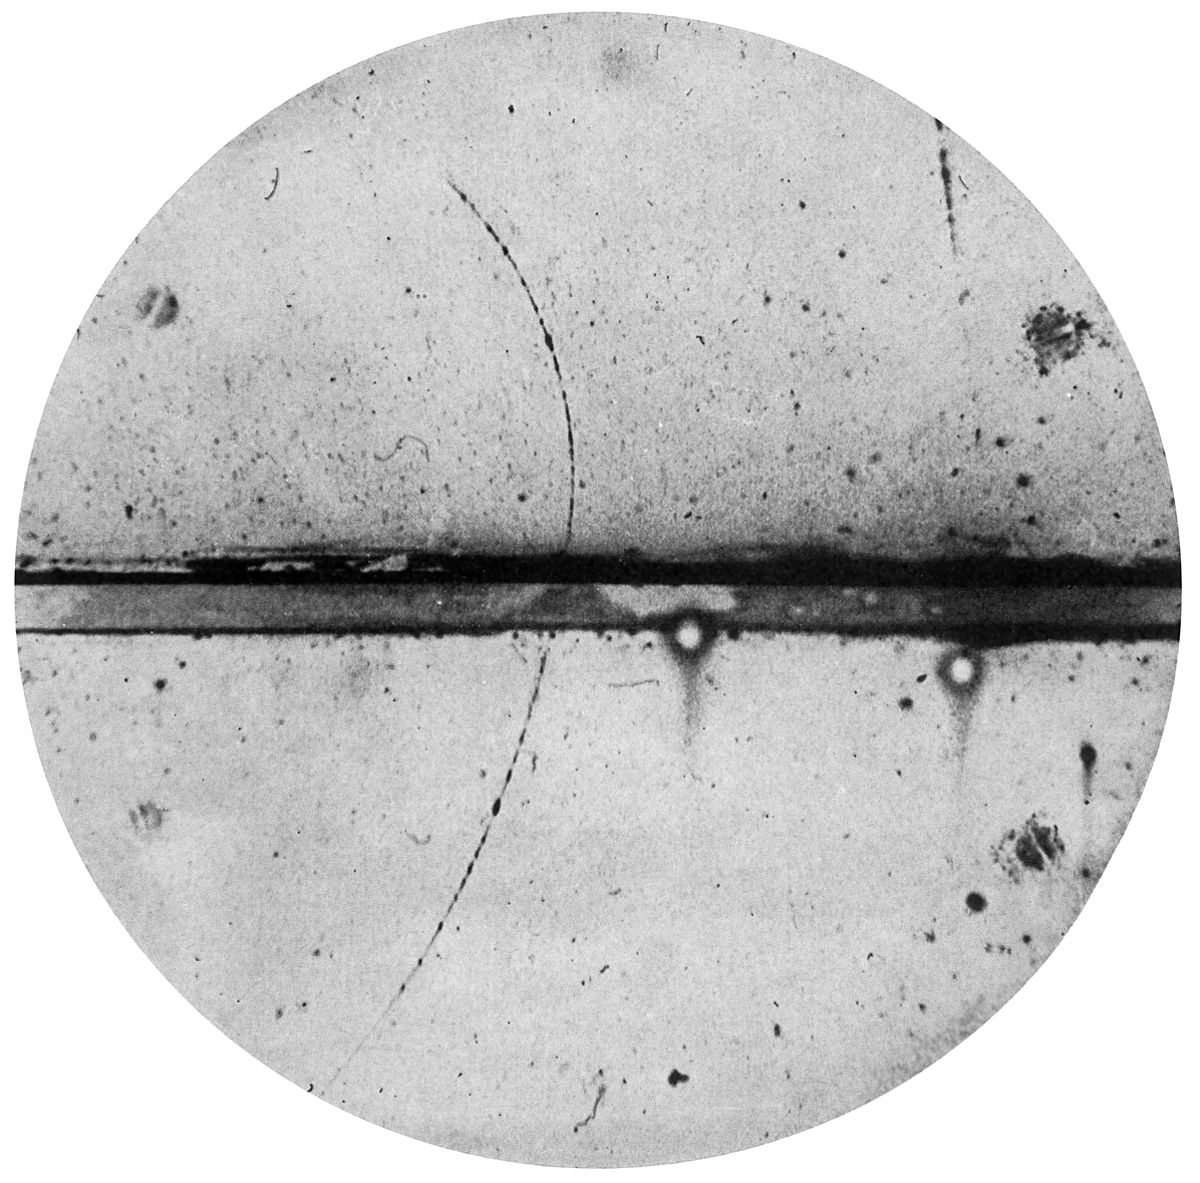
\includegraphics[width=.6\textwidth]{Plots/positron_track.jpg}
        \caption{A photograph of a particle track in a cloud chamber. A \SI{6}{\milli\metre} plate of lead separates the top and bottom halves of the image and the particle track clearly intersects this plate. A magnetic field of \SI{1.5}{\tesla} is applied uniformly, pointing out of the page (\textbf{CHECK THIS}we have assumed this as we are told the particle is a positron and can deduce the direction of movement from the fact the radius of curvature decreases from bottom to top, meaning the momentum decreases). }
        \label{fig:positron_track}
    \end{center}
\end{figure}


\newpage
\printbibliography


\end{document}